\section{Rechnerisch den \ce{CO2}-Gehalt und die Luftwechselzahl bestimmen}

Um die \ce{CO2}-Konzentration mit bekannter Luftwechselzahl zu bestimmen ergibt sich mit der Hintergrundbelastung an \ce{CO2} aus der Umgebungsluft folgender Term:

\begin{flalign}
	\label{gl:co2}
	c_{\ce{CO2}} (t) &= c_{\ce{CO2}, \text{außen}} + \frac{N*\dot{V}_{\ce{CO2}}}{10*n*V}*\left[1-e^{-n*t}\right]
\end{flalign}

\begin{flalign}
	\label{gl:luftwechsel}
	n &= \frac{N*\dot{V}_{\ce{CO2}}}{10*V*\left[c_{\ce{CO2}}(t\rightarrow \infty)-c_{\ce{CO2},\text{außen}}\right]}
\end{flalign}

\begin{description}
	\item [$ \boldmath c_{\ce{CO2}} (t) \ldots$] Innenraum Konzentration an \ce{CO2} in Vol.\% zu einem \hspace{10mm} Zeitpunkt t
	\item [$\boldmath c_{\ce{CO2},\text{außen}}\ldots$] Außenkonzentration an \ce{CO2} in Vol.\% ($\approx $ 0,04 Vol.\%)
	\item [$ \boldmath c_{\ce{CO2}} (t\rightarrow \infty)\ldots$] Grenzkonzentration an \ce{CO2} für $t \rightarrow \infty$
	\item[$ \boldsymbol N\ldots$] Anzahl der Personen
	\item[$\boldsymbol n\ldots$] Luftwechselzahl in \si{\per \hour}
	\item[$\boldsymbol V\ldots$] Raumvolumen in \si{\kmeter}
	\item[$\boldmath \dot{V}_{\ce{CO2}}\ldots$] spezifische Emissionsrate in \si{\liter \per \hour}
	\item[$\boldsymbol t\ldots$] Zeit in \si{\hour}
\end{description}
\textit{Es gilt zu beachten, dass diese Gleichungen empirisch sind. So muss beachtet werden, dass die Gleichung nicht Einheiten gerecht ist und somit die Zahlenwerte der definierten Variablen zu nutzen sind !}

\subsection*{Herleitung der Gleichung für die \ce{CO2}-Konzentration}

Um die Gleichung \ref{gl:co2} herzuleiten, ist es nötig den Sachverhalt zu vereinfachen \mbox{(siehe Abb. \ref{fig:kompart})}. Die Blackbox stellt dabei den vereinfachten, betrachteten Raum dar in welchem der \ce{CO2}-Gehalt zum Zeitpunkt $t$ bestimmt werden soll.

\begin{figure}[h!]
	\centering
	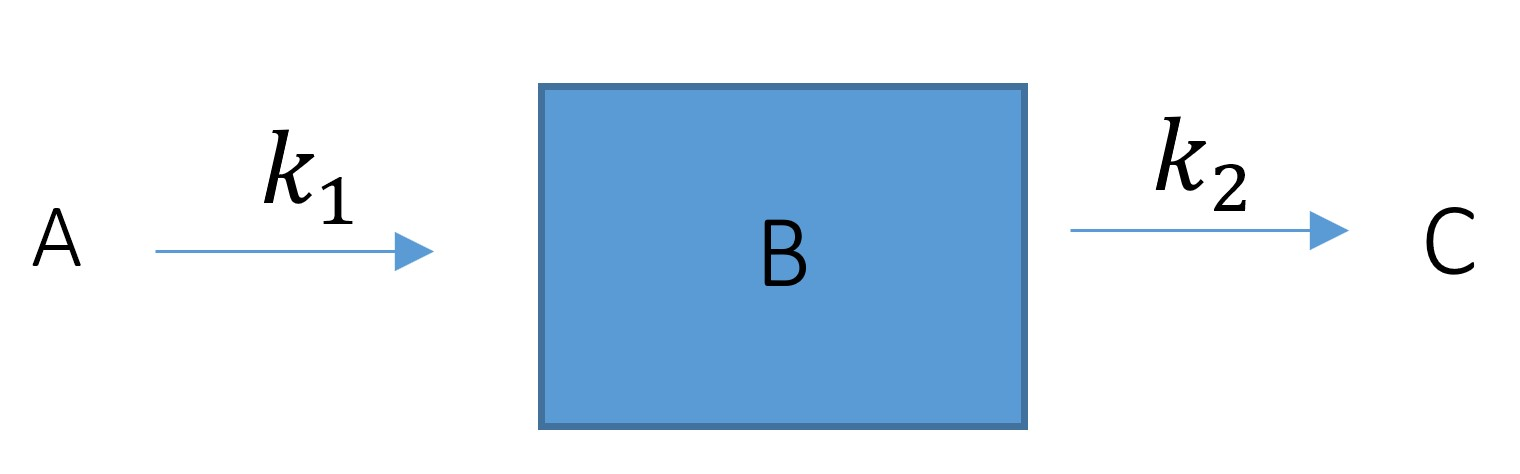
\includegraphics[width=0.8\textwidth]{img/kompart}
	\caption{"'Blackbox"'-Modell für \ce{CO2}-Gehalt eines Raumes}
	\label{fig:kompart}
\end{figure}
\FloatBarrier
%Ende
\begin{description}
	\item[$k_1\ldots$] Geschwindigkeitskonstante des eingehenden Stoffstromes A
	\item[$k_2\ldots$] Geschwindigkeitskonstante des ausgehenden Stoffstromes C
	\item[$A\ldots$] eingehender Stoffstrom A
	\item[$B\ldots$] "`Blackbox"' B
	\item[$C\ldots$]  ausgehender Stoffstrom C
	\item[$c_A\ldots$] Konzentration an \ce{CO2} des eingehenden Stoffstromes A
	\item[$c_B\ldots$] Konzentration an \ce{CO2} der "`Blackbox"' B
	\item[$c_C\ldots$]  Konzentration an \ce{CO2} des ausgehenden Stoffstromes C
\end{description}

Unter der Annahme, dass die Änderung der Konzentration an \ce{CO2} für die Stoffströme A und C konstant bleibt, kann ein differentieller Zusammenhang zwischen den Konzentrationen $c_A$ und $c_C$ jeweils mit der Zeit $t$ aufgestellt werden. Dieser Ausdruck ist unter de folgenden Gleichungen mit den Geschwindigkeitskonstanten $k_1$ und $k_2$ in einen Zusammenhang gebracht worden.
\begin{flalign}
	\dv{c_A}{t} &= - k_1 *c_A
\end{flalign}

\begin{flalign}
	\dv{c_c}{t} &= k_2 *c_B
\end{flalign}

Da A als eingehender Stoffstrom in der Blackbox "`verbraucht"' wird, erhält die Geschwindigkeitskonstante $k_1$ ein negatives Vorzeichen. Die Geschwindigkeitskonstante $k_2$ beschreibt den ausgehenden Stoffstrom , als würde dieser "`produziert"' und erhält somit ein positives Vorzeichen. Da der Stoffstrom C von der Konzentration in der Blackbox abhängig ist, wird hierbei mit der Konzentration $c_B$ gerechnet. Stoffstrom A ist lediglich vom \ce{CO2}-Gehalt außerhalb der Blackbox abhängig und ist somit lediglich abhängig von $c_A$.\\
Aus dem differentiellen Ansatz vom eingehenden Stoffstrom A und dem ausgehenden Stoffstrom B ergibt sich somit die Gleichung \ref{gl:cb}.
\begin{flalign}
	\label{gl:cb}
	\dv{c_B}{t} &= k_1*c_A-k_2*c_B
\end{flalign}
Die Vorzeichen ergeben sich erneut daraus ob die Stoffströme in die Blackbox eingetragen werden (+) oder die Blackbox verlassen (-).
Daraus lässt im folgenden die Gleichung für die \ce{CO2}-Konzentration aus bekannten Daten wie der Personenzahl $N$ oder der Luftwechselzahl $n$ berechnen.
\FloatBarrier

\vspace*{5mm}

\textbf{Umformungen für die Formel der \ce{CO2}-Konzentration in einem Raum in Abhängigkeit von der Zeit:}
\begin{flalign}
		c_b &= \frac{k_1}{k_2}*c_{A,0}*\left(1-e^{-k_2*t}\right)\\
			&= \frac{k_1}{k_2}*c_{A,0}*\left(1-e^{-k_2*t}\right)\\
			&= \frac{\frac{\dot{V}_{\ce{CO2}}}{V}}{k_2}*\frac{N}{10}*\left(1-e^{-k_2*t}\right)\\
			&= \frac{1}{k_2}*\frac{N*\dot{V}_{\ce{CO2}}}{10*V}*\left(1-e^{-k_2*t}\right)\\
	\tag{siehe Gl. \ref{gl:co2}}
	c_{\ce{CO2}, \text{innen}} (t) &= \frac{N*\dot{V}_{\ce{CO2}}}{10*n*V}*\left(1-e^{-n*t}\right) \\
	c_{\ce{CO2}} (t) &= c_{\ce{CO2}, \text{außen}} + \frac{N*\dot{V}_{\ce{CO2}}}{10*n*V}*\left[1-e^{-n*t}\right]	
\end{flalign}
